\begin{exercise}
  Ziel dieser Aufgabe sit die Konstruktion eines Differenzenverfahrens für krumme
  Ränder. Sie dazu $E =(x_ic y_j) \in \R^2 \in \Omega$ ein Gitterpunkt im Inneren
  von $\Omega$, sodass die Gitterpunkte links $(x_i -h, y_j)$ und unterhalb
  $(x_i,y_j -h)$ von $E$ im Gebiet $\Omega$ liegen aber die Gitterpunkte rechts
  $(x_i + h, y_j)$ und oberhalb $(x_i, y_j + h)$ von $E$ nicht mehr in $\Omega$ liegen.
  Konstruieren Sie analog zu Aufgabe $59$ einen $5$-Punkt Differenzenstern für
  $\delta u(E)$, welcher $E$, die in $\Omega$ liegenden Nachbarpunkte $(x_i -h, y_j)$
  und $(x_i, y_j -h)$ sowie die Randpunkte
  $(x_i + \delta_x h , y_j), (x_i, y_j + \delta_y h) \in \partial \Omega$ mit
  $\delta_x, \delta_y \in (0,1)$ verwendet (siehe Abb. $2$). Welche Ordnung kann man
  erreichen?

  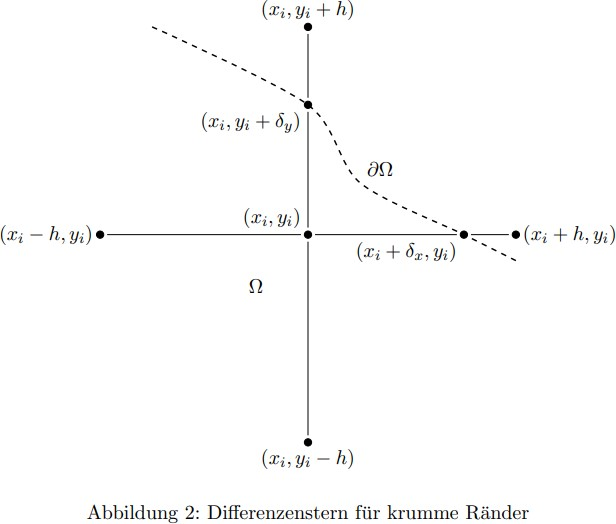
\includegraphics{Abbildung_2}
\end{exercise}

\begin{solution}
  Wie in der vorigen Aufgabe nehmen wir uns ein hinreichend glattes $u$ und entwickeln erstmal

  \begin{align*}
    u(x_i-h,y_i) &= u(x_i,y_i) &- h\partial_x u(x_i,y_i) &+ \frac{h^2}{2}\partial_x^2 u(x_i,y_i) &- \frac{h^3}{6}\partial_x^3 u(x_i,y_i) &+ \Landau{h^4}\\
    u(x_i+h\delta_x,y_i) &= u(x_i,y_i) &+ h\delta_x\partial_x u(x_i,y_i) &+ \frac{h^2 \delta_x^2}{2}\partial_x^2 u(x_i,y_i) &+ \frac{h^3 \delta_x^3}{6}\partial_x^3 u(x_i,y_i) &+ \Landau{h^4}\\
    u(x_i,y_i-h) &= u(x_i,y_i) &- h\partial_y u(x_i,y_i) &+ \frac{h^2}{2}\partial_y^2 u(x_i,y_i) &- \frac{h^3}{6}\partial_y^3 u(x_i,y_i) &+ \Landau{h^4}\\
    u(x_i,y_i+h\delta_y) &= u(x_i,y_i) &+ h\delta_y\partial_y u(x_i,y_i) &+ \frac{h^2 \delta_y^2}{2}\partial_y^2 u(x_i,y_i) &+ \frac{h^3 \delta_y^3}{6}\partial_y^3 u(x_i,y_i) &+ \Landau{h^4}
  \end{align*}

  Wir versuchen zunächst einmal, durch geeignete Kombination der Sternwerte die Terme bis zur Ordnung 3 verschwinden zu lassen (so wie man das im Normalfall tun kann).

  Das Gleichungssystem, das wir hierfür lösen müssen, sieht folgendermaßen aus

  \begin{align*}
    \begin{pmatrix}
      1 & 1 & 1 & 1 & 1 \\
      -1 & \delta_x & 0 & 0 & 0 \\
      0 & 0 & -1 & \delta_y & 0 \\
      -\frac{1}{6} & \frac{\delta_x^3}{6} & 0 & 0 & 0 \\
      0 & 0 & -\frac{1}{6} & \frac{\delta_y^3}{6} & 0 \\
    \end{pmatrix}
    \begin{pmatrix}
      c_{x,-1} \\
      c_{x,1} \\
      c_{y,-1} \\
      c_{y,1} \\
      c_{0}
    \end{pmatrix} =
    \begin{pmatrix}
      0 \\ 0 \\ 0 \\ 0 \\ 0
    \end{pmatrix}
  \end{align*}

  Man sieht, dass die Matrix regulär ist und dieses System somit nur trivial lösbar ist.
  Das heißt wir können die Terme mit Ordnung 3 nicht verschwinden lassen, und müssen uns mit den Termen bis Ordnung 1 begnügen (also nur den ersten 3 Zeilen des Gleichungssystems).

  Eine Lösung hierfür ist offensichtlich gegeben durch

  \begin{align*}
  \begin{pmatrix}
  c_{x,-1} \\
  c_{x,1} \\
  c_{y,-1} \\
  c_{y,1} \\
  c_{0}
  \end{pmatrix} =
  \begin{pmatrix}
    1+\delta_y \\ \frac{1+\delta_y}{\delta_x} \\ 1+\delta_x \\ \frac{1+\delta_x}{\delta_y} \\ -(c_{x,-1}+ c_{x,1} + c_{y,-1} + c_{y,1})
  \end{pmatrix}
  \end{align*}

  und es folgt

  \begin{align*}
  \begin{pmatrix}
  & c_{y,-1} &\\
  c_{x,-1} & c_0 & c_{x,1}\\
  & c_{y,1} &
  \end{pmatrix}
  u(x_i,y_i) &= \frac{h^2}{2}\partial_x^2u(x_i,y_i)(1 + \delta_y + (1+\delta_y)\delta_x ) +\frac{h^2}{2}\partial_y^2 u(x_i,y_i)(1 + \delta_x + (1 + \delta_x)\delta_y) + \Landau{h^3} \\
  &= h^2 \frac{(1 + \delta_x)(1 + \delta_y)}{2} (\partial_x^2 u(x_i,y_i) + \partial_y^2 u(x_i,y_i)) + \Landau{h^3} \\
  &\Rightarrow \Delta u(x_i,y_i) = \frac{1}{h^2} \frac{2}{(1 + \delta_x)(1 + \delta_y)} \begin{pmatrix}
  & c_{y,-1} &\\
  c_{x,-1} & c_0 & c_{x,1}\\
  & c_{y,1} &
  \end{pmatrix} u(x_i,y_i) + \Landau{h}.
  \end{align*}

  (Kann man dann noch vereinfachen)

  Wir erhalten hier also nur Ordnung 1.
\end{solution}
